\subsection{Képek és hivatkozások}

%29
\begin{frame}
  Képeket az \texttt{<img>} üres, soron belüli elemmel adunk meg. Attribútumok:
  \begin{description}[m]
    \item[\texttt{alt}] (alternate text) \hfill \\ Kép leírása (gyengénlátók, szöveges böngészők, stb. számára), kötelező.
    \item[\texttt{src}] (source) \hfill \\ Teljes/relatív elérési útvonal, URL
    \item[\texttt{width}] \hfill \\ Szélesség képpontokban
    \item[\texttt{height}] \hfill \\ Magasság képpontokban
  \end{description}
  Bár a méretet megadó attribútumok nem elavultak, \emph{ajánlott} a méretet CSS-sel megadni (CSS szabályok felülbírálják az attribútumok tartalmát). Az oldalak felesleges újratördelése elkerülhető a méretek megadásával.
\end{frame}

%30
\begin{frame}[fragile]
  Széles körben támogatott formátumok: jpeg, gif, png.
  \vfill
  Képek (\texttt{<img>} elemek) beágyazhatók a \texttt{<figure>} blokk szintű elembe.\\
  Célszerű beágyazni a kép feliratát is \texttt{<figcaption>} elemben.
  \vfill
  Például:
  \begin{verbatim}
<figure>
  <img alt="kep" src="kep.jpeg" width="320" height="240" />
  <figcaption>Az egyetem logoja</figcaption>
</figure>
  \end{verbatim}
\end{frame}

%31
\begin{frame}
  \begin{columns}[c]
    \column{0.85\textwidth}
      Készítse el az alábbi oldalt! Képek adatai:
      \begin{enumerate}
        \item Forrás: \textattachfile{SZElogo.png}{SZElogo.png}, méret: 7088x2363 (kicsinyítse 10\%-ra!)
        \item Forrás: \textattachfile{html.gif}{html.gif}, méret: 500x400
        \item Forrás: \hiv{\href{https://www.w3.org/html/logo/downloads/HTML5\_Logo\_256.png}{https://www.w3.org/html/logo/downloads/HTML5\_Logo\_256.png}}, méret: 256x256
      \end{enumerate}
    \column{0.15\textwidth}
        \begin{center}
          \begin{exampleblock}{\textattachfile{kep.html}{kep.html}}
            \centering 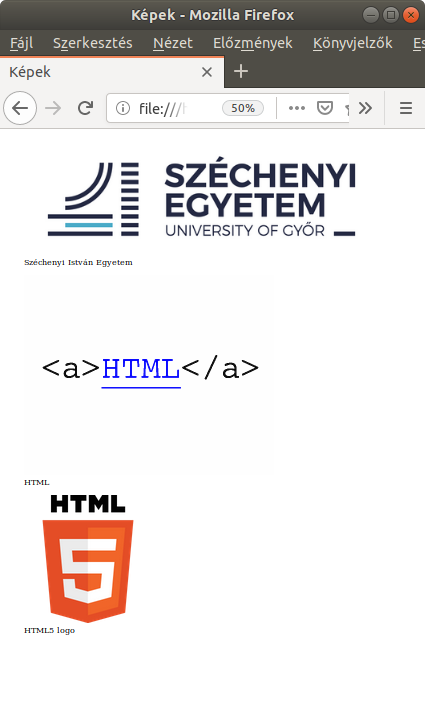
\includegraphics[scale=.14]{kep.png}
          \end{exampleblock}
        \end{center}
  \end{columns}  
\end{frame}

%_
\begin{frame}
  Néha a képfájlokat nem tudjuk/akarjuk feltölteni egy szerverre $\to$ beágyazzuk őket a weboldalba \hiv{\href{https://tools.ietf.org/html/rfc2397}{Data URL}}-ek segítségével:
  \vfill
  \begin{exampleblock}{Általános felépítés}
    \texttt{data:[<mediatype>][;base64],<data>}
  \end{exampleblock}
  \begin{exampleblock}{\textattachfile{dataurl.html}{dataurl.html}}
    \scriptsize
    \texttt{<img src="data:image/svg+xml;base64,PD94bWwgdmV...ZnPg0K" alt="IT logo" width="400" />}
  \end{exampleblock}
  \vfill
  \small
  \begin{itemize}
    \item Nem csak képek forrása adható meg ilyen módon, de ez a leginkább jellemző.
    \item Sok böngészőnél az URL hossza nem haladhatja meg a 64kB-ot.
    \item Base64 kódolást lehet végezni Linuxon/Max OS-en a \hiv{\href{https://linux.die.net/man/1/base64}{base64}} programmal, de vannak \hiv{\href{https://www.base64-image.de/}{online}} \hiv{\href{https://www.base64encode.org/}{eszközök}} is.
  \end{itemize}
\end{frame}

%32
\begin{frame}
  Kis kijelzőre nincs értelme túl nagy képet letölteni, majd összezsugorítani $\to$ eszközfüggő képek letöltése \emph{CSS3 media query} segítségével
  \begin{columns}
    \column{0.7\textwidth}
      \begin{exampleblock}{\textattachfile{kepmeret.html}{kepmeret.html}, \textattachfile{allatok.zip}{képfájlok}}
        \tiny
        \lstinputlisting[style=HTML,linerange={8-15},numbers=left,firstnumber=8]{kepmeret.html}
      \end{exampleblock}
    \column{0.3\textwidth}
      \centering 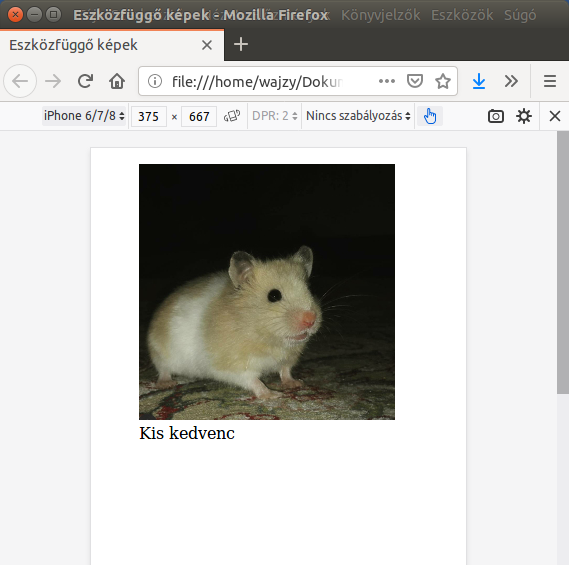
\includegraphics[scale=.18]{kepmeret.png}
  \end{columns} 
  \begin{enumerate}
    \item A böngésző az első, feltételeknek megfelelő képet fogja használni.
    \item Az utolsó beágyazott elem egy \texttt{<img>} legyen! (Kompatibilitás miatt, és alapértelmezett képet is definiál.)
  \end{enumerate}
\end{frame}

%33
\begin{frame}
  \footnotesize
  Hiperhivatkozások készíthetők \texttt{<a>} (anchor) soron belüli elemmel. A nyitó és záró címkék közötti szöveg/kép az érzékeny terület. Attribútumok:
  \begin{description}[m]
    \item[\texttt{href}] (hypertext reference) \hfill \\ Abszolút/relatív útvonal/URL, az ugrás célja. Könyvtár megadás esetén célszerű / jellel zárni.
    \item[\texttt{target}] \hfill \\ Hol nyíljon meg a betöltött tartalom? Értéke lehet:
    \begin{itemize}
      \item \texttt{\_blank} Új ablakban/fülön
      \item \texttt{\_self} Ugyanott, ahol a link is található (alapértelmezés)
      \item \texttt{\_parent} Szülő keretben. (A keretek \kiemel{ELAVULTAK}.)
      \item \texttt{\_top} A teljes ablakban, a keretből ,,kitörve''. (A keretek \kiemel{ELAVULTAK}.)
      \item \emph{keretnév} Adott nevű keretben. (A keretek \kiemel{ELAVULTAK}.)
    \end{itemize}
    \item[\texttt{title}] \hfill \\ Tooltip szöveg
  \end{description}
  Például: \texttt{<a href="https://www.google.com/">Ugrás a kereső oldalára</a>}
\end{frame}

%34
\begin{frame}
  \begin{columns}[c]
    \column{0.5\textwidth}
      Az ábrának megfelelően készítsen három hivatkozást egymás alatti bekezdésekben!
      \begin{itemize}
        \item A Széchenyi Egyetem oldalát az aktuális oldal helyére kell betölteni,
        \item az Edutusét új ablakba/fülre! 
        \item Végül a \textattachfile{HTML5sticker.png}{HTML5sticker.png} képet használva lehessen eljutni a W3C oldalára!
      \end{itemize}
      Készítsen feliratokat (SZE, Edutus, HTML5), melyek megjelennek az egeret a link fölé mozgatva!
    \column{0.5\textwidth}
      \begin{center}
        \begin{exampleblock}{\textattachfile{hivatkozas.html}{hivatkozas.html}}
          \centering 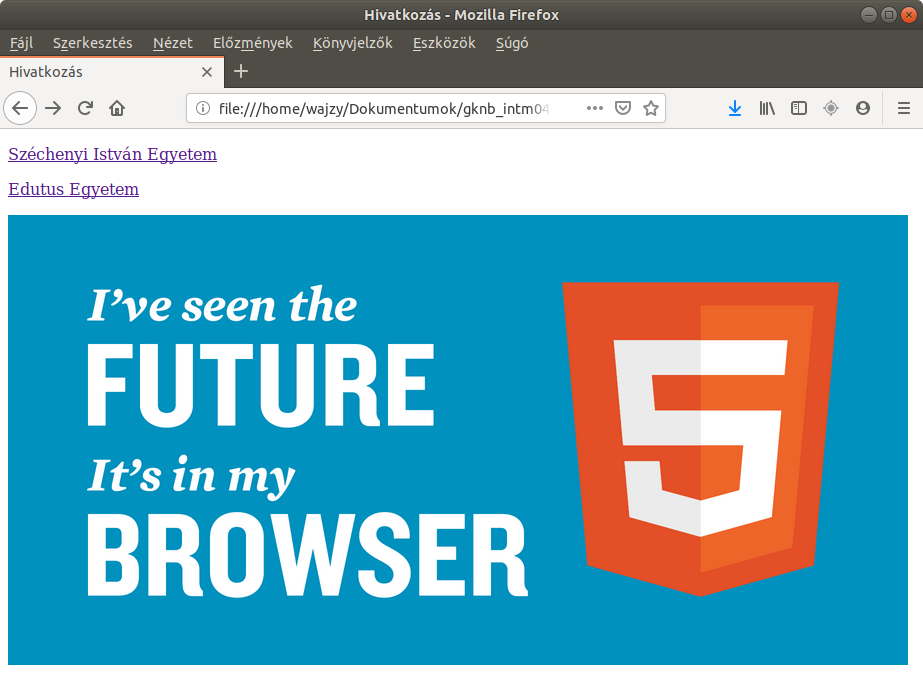
\includegraphics[scale=.2]{hivatkozas.png}
        \end{exampleblock}
      \end{center}
  \end{columns}
\end{frame}

%35
\begin{frame}
  \begin{columns}[c]
    \footnotesize
    \column{0.65\textwidth}
      Oldalon belülre mutató hivatkozások is készíthetők, főleg hosszú dokumentumokhoz.
      \begin{enumerate}
        \item Egyedi azonosító készítése az ugrás céljához \texttt{id} (globális) attribútummal, pl.: \texttt{<h1 id="egy">Első fejezet</h1>}
        \item Hivatkozás (\texttt<a> elem) készítése, a \texttt{href} attribútum értékét \#-tel kell kezdeni, majd az azonosítóval folytatni, pl. \texttt{<a href="\#egy">Ugrás az 1. fejezetre</a>}
      \end{enumerate}
      \vfill
      A \textattachfile{jonas.txt}{jonas.txt} fájlból kiindulva hozza létre az ábrán látható oldalt! Az első sor első szintű címsor, a tartalomjegyzék felirat és a vers egyes részei második szintűek. A vers bekezdései bekezdésként jelöltek. A tartalomjegyzék soraira kattintva lehessen elugrani a megfelelő versszakig!
    \column{0.35\textwidth}
      \begin{center}
        \begin{exampleblock}{\textattachfile{jonas.html}{jonas.html}}
          \centering 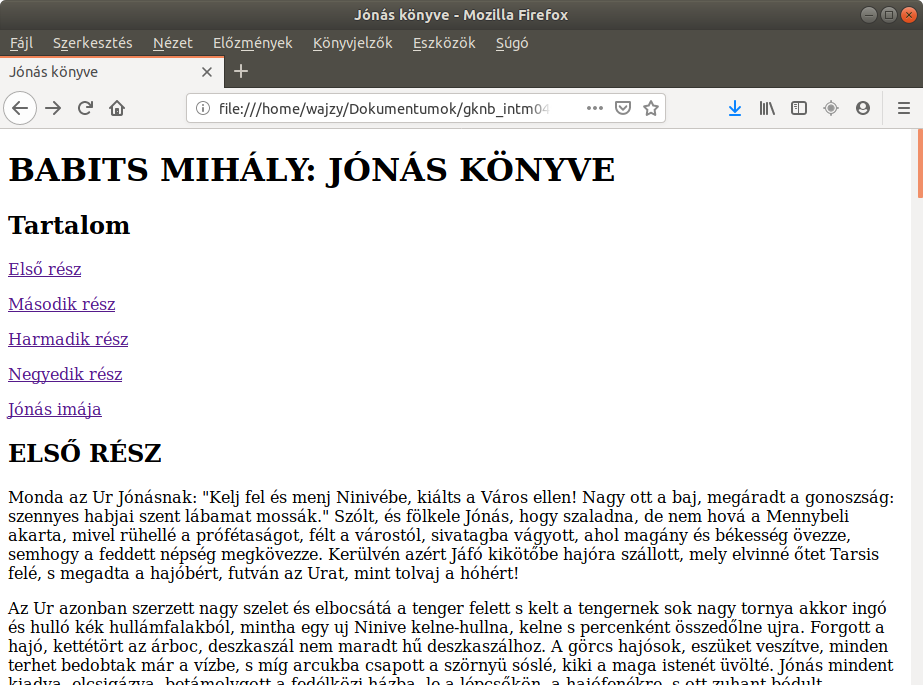
\includegraphics[scale=.15]{jonas.png}
        \end{exampleblock}
      \end{center}
  \end{columns}
\end{frame}

%36
\begin{frame}
  Kép egyes részei kijelölhetők, és más-más oldalakra hivatkozhatnak.
  \begin{enumerate}
    \item Megjeleníteni a képet \texttt{<img>} elemmel, elhelyezni benne a \texttt{usemap} attribútumot, melynek értéke \#-tel kezdődik, és a \emph{térkép} nevével folytatódik.
    \item Létrehozni valahol egy \texttt{<map>} elemet, melynek \texttt{name} attribútuma tartalmazza a térkép nevét.
    \item Ebbe beágyazni \texttt{<area>} üres elemeket, melynek \texttt{shape} attribútuma egy alakzatot, \texttt{coords} attribútuma pedig ennek koordinátáit definiálja:
    \begin{itemize}
      \item \texttt{rect} téglalap, két átellenes sarok X, Y koordinátájával
      \item \texttt{circle} kör, középpont X, Y koordinátája, sugár
      \item \texttt{poly} poligon, egymást követő pontok x, Y koordinátái; az utolsót összeköti az elsővel
      \item \texttt{default} a teljes kép külön nem jelölt része
    \end{itemize}
    \item Az \texttt{<area>} \texttt{href} attribútuma definiálja a célt.
  \end{enumerate}
\end{frame}

%37
\begin{frame}
  A \textattachfile{cyclist.jpg}{cyclist.jpg} felhasználásával hozza létre a \textattachfile{terkepek.html}{terkepek.html} weboldalt! A képen kijelölendő területek alakja, koordinátái és célja az alábbi:
  
    \begin{table}
      \resizebox{\textwidth}{!}{
      \begin{tabular}{llp{3cm}l}
      Mit jelöl ki? & Alakzat  & Koordináták                                                                                     & Cél                                                            \\ \hline
      Első kereket  & Kör      & 217, 813, 145                                                                                     & https://ebike.hu/termekek/kerek/felni/                         \\
      Kosarat       & Téglalap & 102, 420, 256, 643                                                                                 & https://ebike.hu/termekek/kiegeszitok/csomagtarto/elore/       \\
      Gyerekülést   & Poligon  & 895, 346, 859, 409, 841, 480, 774, 507, 744, 579, 771, 690, 742, 732, 832, 724, 813, 606, 873, 589, 873, 466, 915, 358 & https://ebike.hu/termekek/kiegeszitok/gyermekules/hatra-vazra/ \\
      Maradék részt & ~        & ~                                                                                               & https://ebike.hu/                                              \\
      \end{tabular}
      }
    \end{table}
\end{frame}

%38
\begin{frame}
  Szerver oldali térképek\\
  A kattintás helyét küldi a szervernek URL-be kódolva.
  \begin{enumerate}
    \item Hozzunk létre hivatkozást a webhelyre! (\texttt{<a>} elem)
    \item Ágyazzuk bele a képet (\texttt{<img>}) az \texttt{ismap} attribútummal!
  \end{enumerate}
  Például: \texttt{<a href="weblap.html"><img alt="Kép" src="kep.jpeg" ismap="ismap"></a>}
  \vfill
  Feladat: alakítsa át az előző feladatot szerver oldali térképet használóra! (\textattachfile{terkepSzerver.html}{Megoldás})
\end{frame}
